\chapter{Advanced Topics}
\label{chap:advanced_topics}

In this chapter, we have tried to collect and document a series of advanced topics related to eMoflon and EA.
It is kept rather compact and is meant to be used mainly as a reference, to be consulted on demand when you need it.

\section{Using Enterprise Architect with Subversion}
The following steps are required to setup EA for use with subversion.
This is highly recommended when working in a group and sharing a single EA Project (EAP) file, which is otherwise a huge binary blob.
We assume you wish to use (i) Subversion and (ii) Windows.
For other SCM and operating systems please consult the official documentation from EA.

Download and install Slik SVN (mandatory):
\begin{enumerate}
  \item[$\blacktriangleright$] x32: \small{\url{http://www.sliksvn.com/pub/Slik-Subversion-1.6.17-win32.msi}}\\\\
   x64: {\small \url{http://www.sliksvn.com/pub/Slik-Subversion-1.6.17-x64.msi}}
\end{enumerate}

For public/private key authentication, you also need Tortoise SVN:
 
\begin{enumerate}
  \item[$\blacktriangleright$] x32: {\small \begin{minipage}{.95\textwidth}  \url{http://sourceforge.net/projects/tortoisesvn/files/1.6.16/Application/TortoiseSVN-1.6.16.21511-win32-svn-1.6.17.msi/download}
    \end{minipage}}\\\\\\
  x64: {\small\begin{minipage}{.9\textwidth}  \url{http://sourceforge.net/projects/tortoisesvn/files/1.6.16/Application/TortoiseSVN-1.6.16.21511-x64-svn-1.6.17.msi/download}\end{minipage}}
\end{enumerate}

If you do not want to have your private key password in plain text in an SVN configuration file then also download Pageant:
\begin{enumerate}
  \item[$\blacktriangleright$] {\small \url{http://the.earth.li/~sgtatham/putty/latest/x86/pageant.exe}}  
\end{enumerate}

After installing all the tools we need, we now have to setup the SSH tunnel:
   
\begin{enumerate}
  \item[$\blacktriangleright$] Locate the file \texttt{\%APPDATA\%$\backslash$Subversion$\backslash$config} and open it with your favourite editor. Locate the \texttt{[tunnels]} section.
  \item[$\blacktriangleright$] If you do not want to install Pageant and do not mind entering your password in plain text enter the following command:\\
  \texttt{ssh = "<path to Tortoise SVN>/bin/TortoisePlink.exe" -l \\<username> -pw <password for your private key> -i "<path to your private key>"}
  \item[$\blacktriangleright$] If you wish to use Pageant then the command can be simplified to:\\ \texttt{ssh = "<path to Tortoise SVN>/bin/TortoisePlink.exe" -l \\<username>} as you can add your private key to Pageant.
  \item[$\blacktriangleright$] If you just use direct passwords for authentication then you can leave out the \texttt{-i} option in both cases.
\end{enumerate}


The next step is to register an SVN-variable in EA:
\begin{enumerate}
  \item[$\blacktriangleright$] Open a model, right click on a root folder and select ``Package Control'' and then ``Version Control Settings...'' (Fig.~\ref{fig:advanced-topics-eaSVN-rightclick}).
  \item[$\blacktriangleright$] In the dialogue, choose a unique ID of your choice (we suggest you use the name of the EAP file) for the settings and activate the ``Subversion'' radio button below.
  \item[$\blacktriangleright$] Choose the local path to the folder which contains the EAP file in the ``Working Copy Path'' text-box.
  \item[$\blacktriangleright$] The field ``Working Station'' must point to where you installed Sliksvn, i.e., \texttt{<path to SlikSVN>$\backslash$bin$\backslash$svn.exe")}.  
  Press ``Save'' and close the dialogue.
  If the dialogue closes without an error message, then you can be sure to have configured everything correctly.
\end{enumerate}
 
%\usepackage{graphics} is needed for \includegraphics
\begin{figure}[htbp]
\begin{center}
	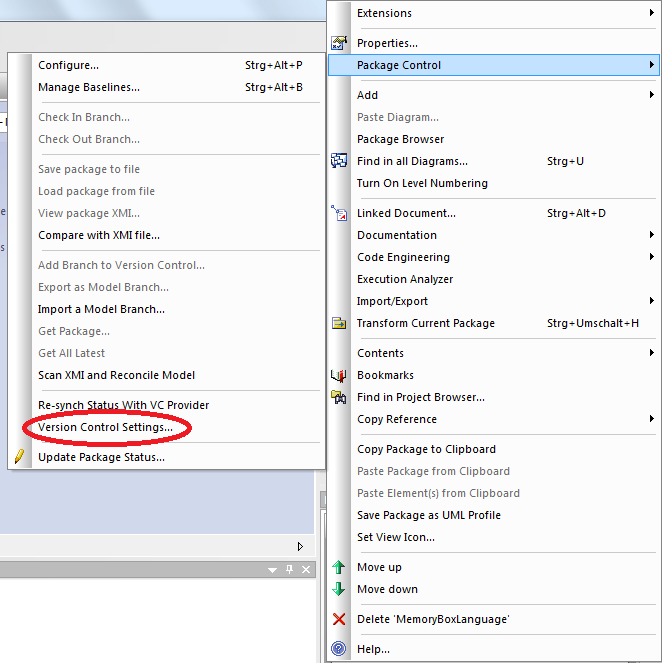
\includegraphics[height=0.45\textheight]{pics/advancedTopics/eaSVN/rightclick.png}\\	
	\vspace{0.5 cm}
	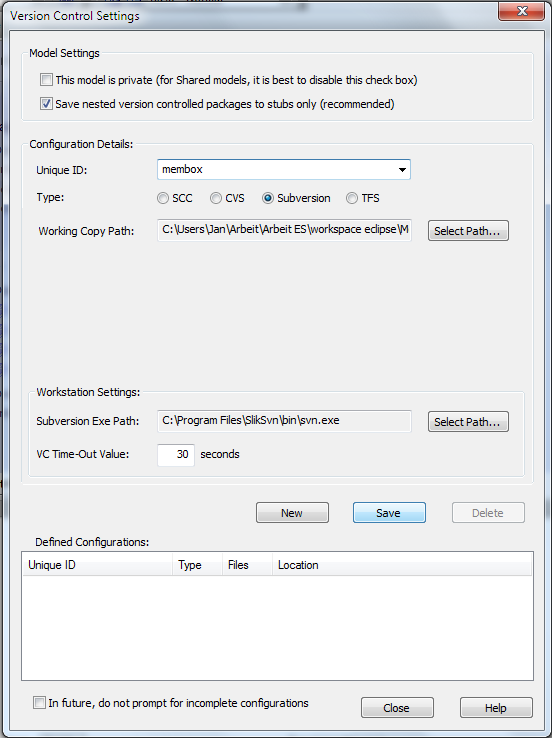
\includegraphics[height=0.45\textheight]{pics/advancedTopics/eaSVN/versioncontrol.png}
	\caption{Register an SVN variable in EA}
  	\label{fig:advanced-topics-eaSVN-rightclick}
\end{center}
\end{figure}

\subsection{How to set-up and work with an EAP file that is already under version control}

\begin{enumerate}
  \item[$\blacktriangleright$] Check out the project with the EAP file from the server using Tortoise-SVN or Eclipse/Subclipse. 
  You should now have a \textit{.svn}-folder in the directory where you saved the revision.
  \item[$\blacktriangleright$] Open the EAP file in EA and inspect the model tree. 
  It should somehow resemble Fig.~\ref{fig:advanced-topics-eaSVN-initial}.
  Note that this does not mean that an empty project was checked in, but only that packages have to be checked out explicitly.
\begin{figure}[!htbp]
\begin{center}
	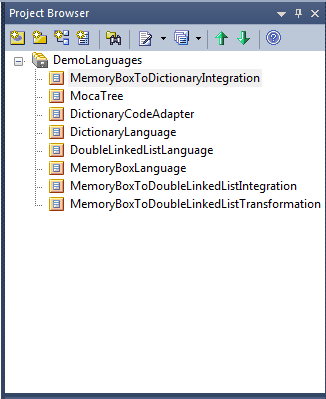
\includegraphics[width=0.5\textwidth]{pics/advancedTopics/eaSVN/DemoLanguages/001.png}
	\caption{Initial state of EAP file}
  	\label{fig:advanced-topics-eaSVN-initial}
\end{center}
\end{figure}

\item[$\blacktriangleright$] To accomplish this make sure you have defined an SVN variable in EA as described in the previous section. 
Now invoke the context menu on the root element and select ``Package Control/Get Package...''~(Fig.~\ref{fig:advanced-topics-eaSVN-getpackage}).
\begin{figure}[!ht]
\begin{center}
	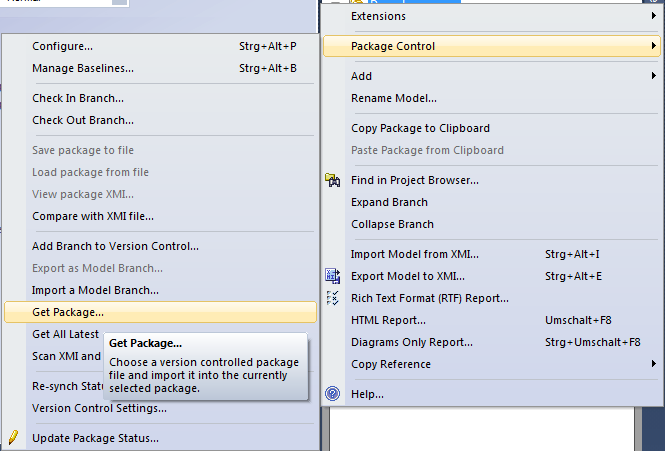
\includegraphics[width=0.9\textwidth]{pics/advancedTopics/eaSVN/DemoLanguages/004.png}
	\caption{``Getting'' a package from the repository}
  	\label{fig:advanced-topics-eaSVN-getpackage}
\end{center}
\end{figure}

 \item[$\blacktriangleright$] Select the \texttt{<package>.xml} with the same name as your root element. 
 In our case, \texttt{DemoLanguages.xml} as depicted in Fig.~\ref{fig:advanced-topics-eaSVN-selectxml}.
\begin{figure}[htbp]
\begin{center}
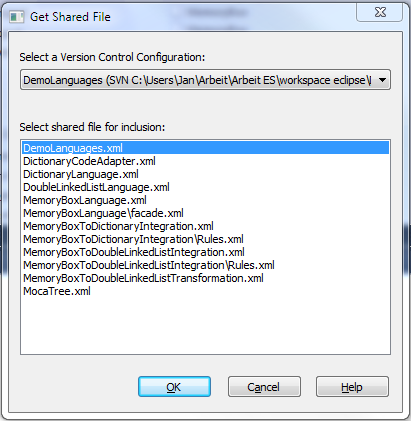
\includegraphics[height=0.5\textheight]{pics/advancedTopics/eaSVN/DemoLanguages/005.png}
	\caption{Choose the correct xml file}
  	\label{fig:advanced-topics-eaSVN-selectxml}
\end{center}
\end{figure}
The key symbol ``8'' beside the folder icon indicates that all packages are under version control and that they are all locked~(Fig.~\ref{fig:advanced-topics-eaSVN-locked}).

\item[$\blacktriangleright$] To retrieve the contents of the project's subpackages do the following:
\begin{enumerate}
\item[1.] \texttt{Check Out} the package you desire (Fig.~\ref{fig:advanced-topics-eaSVN-checkout})
\item[2.] Select \texttt{Get Package} for the package (Fig.~\ref{fig:advanced-topics-eaSVN-getpackage}) and choose the correct XML file (Fig.~\ref{fig:advanced-topics-eaSVN-selectxml}).
\item[3.] All data for this package is now retrieved from the XML file and afterwards also available in your EA browser.
\end{enumerate}
Repeat Steps 1 to 2 for all packages \emph{and} sub-packages (unfortunately also transitively) you wish to work with. 
The good news is that after this initial configuration overhead, only \texttt{Get All Latest} has to be invoked to update all your models. 
More information about updating and checking in changes can be found in the next Section~\ref{sect:appendixB_update_commit}. 
\begin{figure}[htbp]
\begin{center}
	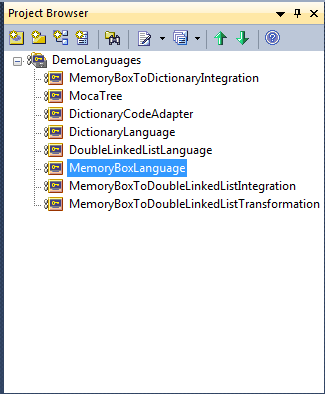
\includegraphics[width=0.4\textwidth]{pics/advancedTopics/eaSVN/DemoLanguages/006.png}
	\caption{Locked packages in EAP file}
  	\label{fig:advanced-topics-eaSVN-locked}
\end{center}
\end{figure}

\begin{figure}[htbp]
\begin{center}
	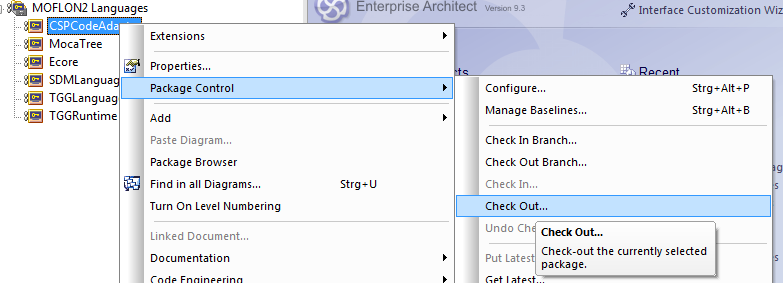
\includegraphics[width=0.9\textwidth]{pics/advancedTopics/eaSVN/checkout.png}
	\caption{Check out of a package}
  	\label{fig:advanced-topics-eaSVN-checkout}
\end{center}
\end{figure}
\begin{figure}[htbp]
\begin{center} 
	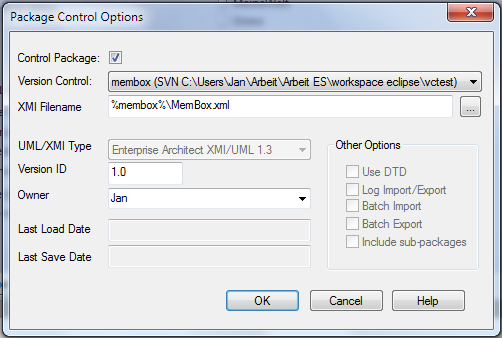
\includegraphics[scale=0.65]{pics/advancedTopics/eaSVN/cont.png}
	\caption{Placing a package under version control}
  	\label{fig:advanced-topics-eaSVN-addPackage}
\end{center}
\end{figure}

\end{enumerate}
 
\subsection{Check Out/Check In vs. Put/Get}
\label{sect:appendixB_update_commit}

\begin{enumerate}
  \item[$\blacktriangleright$] A \texttt{Check Out} retrieves the lock for a model and gives you exclusive access to the package, i.e., no one else can change the model. 
  Very important, if subpackages are also under version control, they are not affected by checking out the ``super''-package and remain locked.
  A \texttt{Check Out} also updates the package to the latest version.

\item[$\blacktriangleright$] A \texttt{Check In} commits your work to the server and gives up the lock on the package so others can work on it.
If you do not want to commit your changes, you can just use \texttt{Undo Check Out...} to revert all local changes.

\item[$\blacktriangleright$]  The corresponding \texttt{..Branch} options perform the actions for the current package and all subpackages.
Please note, this has nothing to do with ``branching'' in normal SVN lingo.

\item[$\blacktriangleright$] \texttt{Get Latest/Get All Latest} retrieves the latest version of the selected package / all packages. 
This is basically an update but does not retrieve the lock for any package.

\item[$\blacktriangleright$] Conversely, \texttt{Put Latest} saves all your changes without giving up any locks.

\item[$\blacktriangleright$] \texttt{Compare with controlled version} can be used to review incoming changes. 
Green elements will be added, red will be deleted. 

\item[$\blacktriangleright$] \texttt{File History} gives you a summary of all commits made while you were lying on the beach. 
For a useful file history, always use meaningful commit statements when checking in! 
A date stamp is created automatically.
\end{enumerate}

\subsection{Placing a package under version control}

\begin{enumerate}

\item[$\blacktriangleright$] If you already have a model in EA and would like to place it under version control, you first have to check it in as usual on the server using your favourite SVN client. 
If the project is already checked in, the required .svn folder should already be in the folder containing the EAP file.

\item[$\blacktriangleright$] In EA, create your SVN variable as described previously and choose ``Package Control$\backslash$Configure...'' for each package you wish to place under version control. 

\item[$\blacktriangleright$] In the ensuing dialogue, activate ``Control Package'' and select your SVN variable from the drop-down menu. 
Enter the path where the XML file for the project should be placed.
Although this is not enforced in any way, we recommend you create a folder structure that mirrors the package structure in EA (Fig.~\ref{fig:advanced-topics-eaSVN-addPackage}).
This process has to be repeated for all sub-packages as soon as their super-package has been placed under version control.
\end{enumerate}

